% Options for packages loaded elsewhere
\PassOptionsToPackage{unicode}{hyperref}
\PassOptionsToPackage{hyphens}{url}
\PassOptionsToPackage{dvipsnames,svgnames,x11names}{xcolor}
%
\documentclass[
  letterpaper,
  DIV=11,
  numbers=noendperiod]{scrreprt}

\usepackage{amsmath,amssymb}
\usepackage{iftex}
\ifPDFTeX
  \usepackage[T1]{fontenc}
  \usepackage[utf8]{inputenc}
  \usepackage{textcomp} % provide euro and other symbols
\else % if luatex or xetex
  \usepackage{unicode-math}
  \defaultfontfeatures{Scale=MatchLowercase}
  \defaultfontfeatures[\rmfamily]{Ligatures=TeX,Scale=1}
\fi
\usepackage{lmodern}
\ifPDFTeX\else  
    % xetex/luatex font selection
\fi
% Use upquote if available, for straight quotes in verbatim environments
\IfFileExists{upquote.sty}{\usepackage{upquote}}{}
\IfFileExists{microtype.sty}{% use microtype if available
  \usepackage[]{microtype}
  \UseMicrotypeSet[protrusion]{basicmath} % disable protrusion for tt fonts
}{}
\makeatletter
\@ifundefined{KOMAClassName}{% if non-KOMA class
  \IfFileExists{parskip.sty}{%
    \usepackage{parskip}
  }{% else
    \setlength{\parindent}{0pt}
    \setlength{\parskip}{6pt plus 2pt minus 1pt}}
}{% if KOMA class
  \KOMAoptions{parskip=half}}
\makeatother
\usepackage{xcolor}
\setlength{\emergencystretch}{3em} % prevent overfull lines
\setcounter{secnumdepth}{5}
% Make \paragraph and \subparagraph free-standing
\ifx\paragraph\undefined\else
  \let\oldparagraph\paragraph
  \renewcommand{\paragraph}[1]{\oldparagraph{#1}\mbox{}}
\fi
\ifx\subparagraph\undefined\else
  \let\oldsubparagraph\subparagraph
  \renewcommand{\subparagraph}[1]{\oldsubparagraph{#1}\mbox{}}
\fi

\usepackage{color}
\usepackage{fancyvrb}
\newcommand{\VerbBar}{|}
\newcommand{\VERB}{\Verb[commandchars=\\\{\}]}
\DefineVerbatimEnvironment{Highlighting}{Verbatim}{commandchars=\\\{\}}
% Add ',fontsize=\small' for more characters per line
\usepackage{framed}
\definecolor{shadecolor}{RGB}{241,243,245}
\newenvironment{Shaded}{\begin{snugshade}}{\end{snugshade}}
\newcommand{\AlertTok}[1]{\textcolor[rgb]{0.68,0.00,0.00}{#1}}
\newcommand{\AnnotationTok}[1]{\textcolor[rgb]{0.37,0.37,0.37}{#1}}
\newcommand{\AttributeTok}[1]{\textcolor[rgb]{0.40,0.45,0.13}{#1}}
\newcommand{\BaseNTok}[1]{\textcolor[rgb]{0.68,0.00,0.00}{#1}}
\newcommand{\BuiltInTok}[1]{\textcolor[rgb]{0.00,0.23,0.31}{#1}}
\newcommand{\CharTok}[1]{\textcolor[rgb]{0.13,0.47,0.30}{#1}}
\newcommand{\CommentTok}[1]{\textcolor[rgb]{0.37,0.37,0.37}{#1}}
\newcommand{\CommentVarTok}[1]{\textcolor[rgb]{0.37,0.37,0.37}{\textit{#1}}}
\newcommand{\ConstantTok}[1]{\textcolor[rgb]{0.56,0.35,0.01}{#1}}
\newcommand{\ControlFlowTok}[1]{\textcolor[rgb]{0.00,0.23,0.31}{#1}}
\newcommand{\DataTypeTok}[1]{\textcolor[rgb]{0.68,0.00,0.00}{#1}}
\newcommand{\DecValTok}[1]{\textcolor[rgb]{0.68,0.00,0.00}{#1}}
\newcommand{\DocumentationTok}[1]{\textcolor[rgb]{0.37,0.37,0.37}{\textit{#1}}}
\newcommand{\ErrorTok}[1]{\textcolor[rgb]{0.68,0.00,0.00}{#1}}
\newcommand{\ExtensionTok}[1]{\textcolor[rgb]{0.00,0.23,0.31}{#1}}
\newcommand{\FloatTok}[1]{\textcolor[rgb]{0.68,0.00,0.00}{#1}}
\newcommand{\FunctionTok}[1]{\textcolor[rgb]{0.28,0.35,0.67}{#1}}
\newcommand{\ImportTok}[1]{\textcolor[rgb]{0.00,0.46,0.62}{#1}}
\newcommand{\InformationTok}[1]{\textcolor[rgb]{0.37,0.37,0.37}{#1}}
\newcommand{\KeywordTok}[1]{\textcolor[rgb]{0.00,0.23,0.31}{#1}}
\newcommand{\NormalTok}[1]{\textcolor[rgb]{0.00,0.23,0.31}{#1}}
\newcommand{\OperatorTok}[1]{\textcolor[rgb]{0.37,0.37,0.37}{#1}}
\newcommand{\OtherTok}[1]{\textcolor[rgb]{0.00,0.23,0.31}{#1}}
\newcommand{\PreprocessorTok}[1]{\textcolor[rgb]{0.68,0.00,0.00}{#1}}
\newcommand{\RegionMarkerTok}[1]{\textcolor[rgb]{0.00,0.23,0.31}{#1}}
\newcommand{\SpecialCharTok}[1]{\textcolor[rgb]{0.37,0.37,0.37}{#1}}
\newcommand{\SpecialStringTok}[1]{\textcolor[rgb]{0.13,0.47,0.30}{#1}}
\newcommand{\StringTok}[1]{\textcolor[rgb]{0.13,0.47,0.30}{#1}}
\newcommand{\VariableTok}[1]{\textcolor[rgb]{0.07,0.07,0.07}{#1}}
\newcommand{\VerbatimStringTok}[1]{\textcolor[rgb]{0.13,0.47,0.30}{#1}}
\newcommand{\WarningTok}[1]{\textcolor[rgb]{0.37,0.37,0.37}{\textit{#1}}}

\providecommand{\tightlist}{%
  \setlength{\itemsep}{0pt}\setlength{\parskip}{0pt}}\usepackage{longtable,booktabs,array}
\usepackage{calc} % for calculating minipage widths
% Correct order of tables after \paragraph or \subparagraph
\usepackage{etoolbox}
\makeatletter
\patchcmd\longtable{\par}{\if@noskipsec\mbox{}\fi\par}{}{}
\makeatother
% Allow footnotes in longtable head/foot
\IfFileExists{footnotehyper.sty}{\usepackage{footnotehyper}}{\usepackage{footnote}}
\makesavenoteenv{longtable}
\usepackage{graphicx}
\makeatletter
\def\maxwidth{\ifdim\Gin@nat@width>\linewidth\linewidth\else\Gin@nat@width\fi}
\def\maxheight{\ifdim\Gin@nat@height>\textheight\textheight\else\Gin@nat@height\fi}
\makeatother
% Scale images if necessary, so that they will not overflow the page
% margins by default, and it is still possible to overwrite the defaults
% using explicit options in \includegraphics[width, height, ...]{}
\setkeys{Gin}{width=\maxwidth,height=\maxheight,keepaspectratio}
% Set default figure placement to htbp
\makeatletter
\def\fps@figure{htbp}
\makeatother
\newlength{\cslhangindent}
\setlength{\cslhangindent}{1.5em}
\newlength{\csllabelwidth}
\setlength{\csllabelwidth}{3em}
\newlength{\cslentryspacingunit} % times entry-spacing
\setlength{\cslentryspacingunit}{\parskip}
\newenvironment{CSLReferences}[2] % #1 hanging-ident, #2 entry spacing
 {% don't indent paragraphs
  \setlength{\parindent}{0pt}
  % turn on hanging indent if param 1 is 1
  \ifodd #1
  \let\oldpar\par
  \def\par{\hangindent=\cslhangindent\oldpar}
  \fi
  % set entry spacing
  \setlength{\parskip}{#2\cslentryspacingunit}
 }%
 {}
\usepackage{calc}
\newcommand{\CSLBlock}[1]{#1\hfill\break}
\newcommand{\CSLLeftMargin}[1]{\parbox[t]{\csllabelwidth}{#1}}
\newcommand{\CSLRightInline}[1]{\parbox[t]{\linewidth - \csllabelwidth}{#1}\break}
\newcommand{\CSLIndent}[1]{\hspace{\cslhangindent}#1}

\KOMAoption{captions}{tableheading}
\makeatletter
\@ifpackageloaded{tcolorbox}{}{\usepackage[skins,breakable]{tcolorbox}}
\@ifpackageloaded{fontawesome5}{}{\usepackage{fontawesome5}}
\definecolor{quarto-callout-color}{HTML}{909090}
\definecolor{quarto-callout-note-color}{HTML}{0758E5}
\definecolor{quarto-callout-important-color}{HTML}{CC1914}
\definecolor{quarto-callout-warning-color}{HTML}{EB9113}
\definecolor{quarto-callout-tip-color}{HTML}{00A047}
\definecolor{quarto-callout-caution-color}{HTML}{FC5300}
\definecolor{quarto-callout-color-frame}{HTML}{acacac}
\definecolor{quarto-callout-note-color-frame}{HTML}{4582ec}
\definecolor{quarto-callout-important-color-frame}{HTML}{d9534f}
\definecolor{quarto-callout-warning-color-frame}{HTML}{f0ad4e}
\definecolor{quarto-callout-tip-color-frame}{HTML}{02b875}
\definecolor{quarto-callout-caution-color-frame}{HTML}{fd7e14}
\makeatother
\makeatletter
\makeatother
\makeatletter
\@ifpackageloaded{bookmark}{}{\usepackage{bookmark}}
\makeatother
\makeatletter
\@ifpackageloaded{caption}{}{\usepackage{caption}}
\AtBeginDocument{%
\ifdefined\contentsname
  \renewcommand*\contentsname{Table of contents}
\else
  \newcommand\contentsname{Table of contents}
\fi
\ifdefined\listfigurename
  \renewcommand*\listfigurename{List of Figures}
\else
  \newcommand\listfigurename{List of Figures}
\fi
\ifdefined\listtablename
  \renewcommand*\listtablename{List of Tables}
\else
  \newcommand\listtablename{List of Tables}
\fi
\ifdefined\figurename
  \renewcommand*\figurename{Figure}
\else
  \newcommand\figurename{Figure}
\fi
\ifdefined\tablename
  \renewcommand*\tablename{Table}
\else
  \newcommand\tablename{Table}
\fi
}
\@ifpackageloaded{float}{}{\usepackage{float}}
\floatstyle{ruled}
\@ifundefined{c@chapter}{\newfloat{codelisting}{h}{lop}}{\newfloat{codelisting}{h}{lop}[chapter]}
\floatname{codelisting}{Listing}
\newcommand*\listoflistings{\listof{codelisting}{List of Listings}}
\makeatother
\makeatletter
\@ifpackageloaded{caption}{}{\usepackage{caption}}
\@ifpackageloaded{subcaption}{}{\usepackage{subcaption}}
\makeatother
\makeatletter
\makeatother
\ifLuaTeX
  \usepackage{selnolig}  % disable illegal ligatures
\fi
\IfFileExists{bookmark.sty}{\usepackage{bookmark}}{\usepackage{hyperref}}
\IfFileExists{xurl.sty}{\usepackage{xurl}}{} % add URL line breaks if available
\urlstyle{same} % disable monospaced font for URLs
\hypersetup{
  pdftitle={Linear Algebra},
  pdfauthor={Aj Averett},
  colorlinks=true,
  linkcolor={blue},
  filecolor={Maroon},
  citecolor={Blue},
  urlcolor={Blue},
  pdfcreator={LaTeX via pandoc}}

\title{Linear Algebra}
\author{Aj Averett}
\date{2023-08-21}

\begin{document}
\maketitle
\renewcommand*\contentsname{Table of contents}
{
\hypersetup{linkcolor=}
\setcounter{tocdepth}{2}
\tableofcontents
}
\bookmarksetup{startatroot}

\hypertarget{linear-algebra}{%
\chapter*{Linear Algebra}\label{linear-algebra}}
\addcontentsline{toc}{chapter}{Linear Algebra}

\markboth{Linear Algebra}{Linear Algebra}

\hypertarget{notation-for-systems-of-linear-equations}{%
\section*{Notation for systems of linear
equations}\label{notation-for-systems-of-linear-equations}}
\addcontentsline{toc}{section}{Notation for systems of linear equations}

\markright{Notation for systems of linear equations}

\textbf{System of Equations}

\[
\begin{cases}
a_{11}x_1 & + &a_{12}x_2 &+ \dots+ & a_{1n}x_n &= b_1 \\
a_{21}x_1 & + &a_{22}x_2 &+ \dots+ & a_{2n}x_n &= b_2 \\
\vdots && \vdots & \ddots & \vdots & \vdots \\
a_{m1}x_1 & + &a_{m2}x_2 &+ \dots+ & a_{mn}x_n &= b_m
\end{cases}
\]

\textbf{Augmented matrix:} \(\begin{bmatrix}A|\vec{b}\end{bmatrix}\)

\[
\left[\begin{array}{@{}cccc|c@{}}
a_{11} & a_{12} & \dots & a_{1n} & b_1 \\
a_{21} & a_{22} & \dots & a_{2n} & b_2 \\
\vdots & \vdots & \ddots & \vdots & \vdots \\
a_{m1} & a_{m2} & \dots & a_{mn} & b_m
\end{array}\right]
\]

\textbf{Vector Equation:}
\(x_1\vec{a_1}+x_2\vec{a_2}+...+x_n\vec{a_n}=\vec{b}\)

\[
x_1
\begin{bmatrix}
a_{11}\\
a_{21}\\
\vdots\\
a_{m1}
\end{bmatrix} +
x_2
\begin{bmatrix}
a_{12}\\
a_{22}\\
\vdots\\
a_{m2}
\end{bmatrix}+
\dots +
x_n
\begin{bmatrix}
a_{1n}\\
a_{2n}\\
\vdots\\
a_{mn}
\end{bmatrix} = 
\begin{bmatrix}
b_1\\
b_2\\
\vdots\\
b_m
\end{bmatrix}
\]

\textbf{Matrix Equation:} \(A\vec{x}=\vec{b}\)

\[
\begin{bmatrix}
a_{11} & a_{12} & \dots & a_{1n} \\
a_{21} & a_{22} & \dots & a_{2n} \\
\vdots & \vdots & \ddots & \vdots \\
a_{m1} & a_{m2} & \dots & a_{mn}
\end{bmatrix} 
\begin{bmatrix}
x_1 \\ 
x_2 \\ 
\vdots \\ 
x_n
\end{bmatrix}=
\begin{bmatrix}
b_1 \\ b_2 \\ \vdots \\ b_m
\end{bmatrix}
\]

\bookmarksetup{startatroot}

\hypertarget{linear-systems}{%
\chapter{Linear Systems}\label{linear-systems}}

\hypertarget{systems-of-linear-equations}{%
\section*{Systems of Linear
Equations}\label{systems-of-linear-equations}}
\addcontentsline{toc}{section}{Systems of Linear Equations}

\markright{Systems of Linear Equations}

\hypertarget{systems-with-a-single-solution}{%
\subsection*{Systems with a Single
Solution}\label{systems-with-a-single-solution}}
\addcontentsline{toc}{subsection}{Systems with a Single Solution}

Below is a \textbf{linear equation}:

\[
\begin{cases}
x_1 - 2x_2 = -1
\end{cases}
\]

\begin{Shaded}
\begin{Highlighting}[]
\ImportTok{import}\NormalTok{ sympy }\ImportTok{as}\NormalTok{ sp}
\ImportTok{import}\NormalTok{ matplotlib.pyplot }\ImportTok{as}\NormalTok{ plt}
\ImportTok{import}\NormalTok{ numpy }\ImportTok{as}\NormalTok{ np}

\CommentTok{\# Declare variables}
\NormalTok{x1, x2 }\OperatorTok{=}\NormalTok{ sp.symbols(}\StringTok{\textquotesingle{}x\_1 x\_2\textquotesingle{}}\NormalTok{)}

\CommentTok{\# Define the equation}
\NormalTok{equation\_1 }\OperatorTok{=}\NormalTok{ sp.Eq(x1 }\OperatorTok{{-}} \DecValTok{2}\OperatorTok{*}\NormalTok{x2, }\OperatorTok{{-}}\DecValTok{1}\NormalTok{)}
\NormalTok{graph\_eq1 }\OperatorTok{=}\NormalTok{ sp.solve(equation\_1, x2)[}\DecValTok{0}\NormalTok{]}

\CommentTok{\# Generate data for plotting}
\NormalTok{x1\_vals }\OperatorTok{=}\NormalTok{ np.linspace(}\OperatorTok{{-}}\DecValTok{10}\NormalTok{, }\DecValTok{10}\NormalTok{, }\DecValTok{400}\NormalTok{)}
\NormalTok{graph\_eq1\_lambdified }\OperatorTok{=}\NormalTok{ sp.lambdify(x1, graph\_eq1)}
\NormalTok{y1\_vals }\OperatorTok{=}\NormalTok{ graph\_eq1\_lambdified(x1\_vals)}

\CommentTok{\# Plotting}
\NormalTok{fig, ax }\OperatorTok{=}\NormalTok{ plt.subplots(figsize}\OperatorTok{=}\NormalTok{(}\DecValTok{7}\NormalTok{, }\DecValTok{6}\NormalTok{))}

\CommentTok{\# Title and labels}
\NormalTok{ax.set\_title(}\StringTok{\textquotesingle{}A single linear equation\textquotesingle{}}\NormalTok{)}
\NormalTok{ax.set\_xlabel(}\StringTok{\textquotesingle{}$x\_1$                                                                                                                            \textquotesingle{}}\NormalTok{)}
\NormalTok{ax.set\_ylabel(}\StringTok{\textquotesingle{}$x\_2$                                                                                                    \textquotesingle{}}\NormalTok{)}

\CommentTok{\# Plot the equation}
\NormalTok{ax.plot(x1\_vals, y1\_vals, label}\OperatorTok{=}\StringTok{\textquotesingle{}$x\_1 {-} 2x\_2 = {-}1$\textquotesingle{}}\NormalTok{, color}\OperatorTok{=}\StringTok{\textquotesingle{}blue\textquotesingle{}}\NormalTok{)}

\CommentTok{\# Move the left and bottom spines to x = 0 and y = 0, respectively}
\NormalTok{ax.spines[}\StringTok{\textquotesingle{}left\textquotesingle{}}\NormalTok{].set\_position(}\StringTok{\textquotesingle{}zero\textquotesingle{}}\NormalTok{)}
\NormalTok{ax.spines[}\StringTok{\textquotesingle{}bottom\textquotesingle{}}\NormalTok{].set\_position(}\StringTok{\textquotesingle{}zero\textquotesingle{}}\NormalTok{)}
\NormalTok{ax.spines[}\StringTok{\textquotesingle{}right\textquotesingle{}}\NormalTok{].set\_color(}\StringTok{\textquotesingle{}none\textquotesingle{}}\NormalTok{)}
\NormalTok{ax.spines[}\StringTok{\textquotesingle{}top\textquotesingle{}}\NormalTok{].set\_color(}\StringTok{\textquotesingle{}none\textquotesingle{}}\NormalTok{)}

\CommentTok{\# Add legend and grid}
\NormalTok{ax.legend()}
\NormalTok{plt.show()}
\end{Highlighting}
\end{Shaded}

\begin{figure}[H]

{\centering 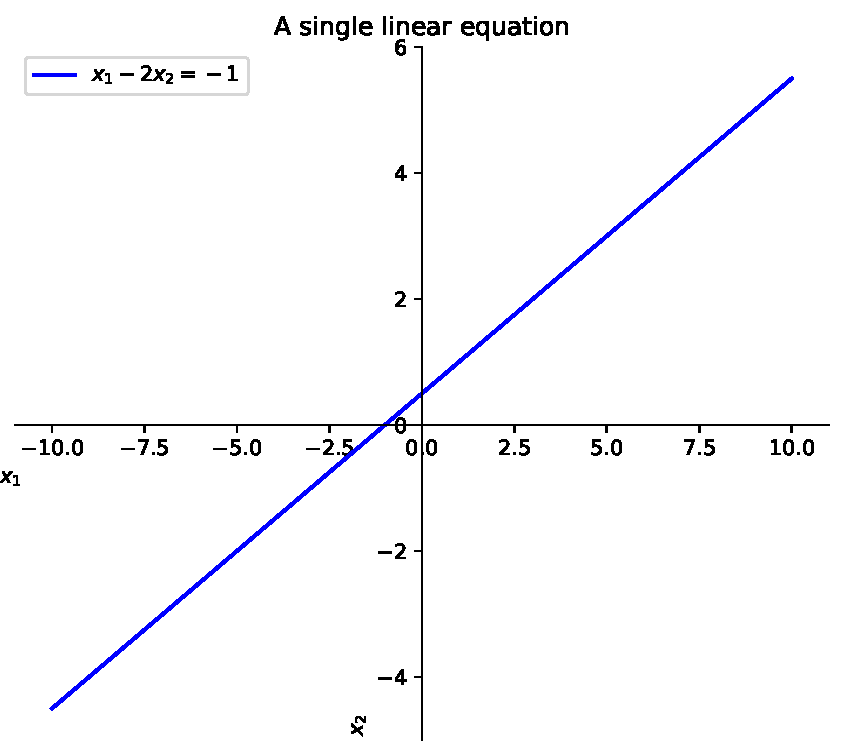
\includegraphics{p1_files/figure-pdf/cell-2-output-1.pdf}

}

\end{figure}

\begin{tcolorbox}[enhanced jigsaw, colbacktitle=quarto-callout-note-color!10!white, toprule=.15mm, colback=white, breakable, titlerule=0mm, leftrule=.75mm, bottomtitle=1mm, opacitybacktitle=0.6, bottomrule=.15mm, title=\textcolor{quarto-callout-note-color}{\faInfo}\hspace{0.5em}{Definition of a linear equation}, left=2mm, colframe=quarto-callout-note-color-frame, rightrule=.15mm, toptitle=1mm, opacityback=0, arc=.35mm, coltitle=black]

A linear equation in the variables \(x_1, x_2, \ldots, x_n\) is an
equation that can be written in the form

\[
a_1x_1 + a_2x_2 + \cdots + a_nx_n = b
\]

where \(b\) and the coefficients \(a_1, a_2, \ldots, a_n\) are real or
complex numbers. The subscript \(n\) may be any positive integer.

\end{tcolorbox}

Take the following \textbf{system of linear equations}: \[
\begin{cases}
&x_1 &- 2x_2 &= -1\\
-&x_1 &+ 3x_2 &= 3
\end{cases}
\]

If we plot these equations on a graph, we can see that they intersect at
a single point. This point is the solution to the system of equations.

\begin{Shaded}
\begin{Highlighting}[]
\ImportTok{import}\NormalTok{ sympy }\ImportTok{as}\NormalTok{ sp}
\ImportTok{import}\NormalTok{ matplotlib.pyplot }\ImportTok{as}\NormalTok{ plt}
\ImportTok{import}\NormalTok{ numpy }\ImportTok{as}\NormalTok{ np}

\NormalTok{x1, x2 }\OperatorTok{=}\NormalTok{ sp.symbols(}\StringTok{\textquotesingle{}x\_1 x\_2\textquotesingle{}}\NormalTok{)}

\NormalTok{equation\_1 }\OperatorTok{=}\NormalTok{ sp.Eq(x1 }\OperatorTok{{-}} \DecValTok{2}\OperatorTok{*}\NormalTok{x2, }\OperatorTok{{-}}\DecValTok{1}\NormalTok{)}
\NormalTok{graph\_eq1 }\OperatorTok{=}\NormalTok{ sp.solve(equation\_1, x2)[}\DecValTok{0}\NormalTok{]}

\NormalTok{equation\_2 }\OperatorTok{=}\NormalTok{ sp.Eq(}\OperatorTok{{-}}\NormalTok{x1 }\OperatorTok{+} \DecValTok{3}\OperatorTok{*}\NormalTok{x2, }\DecValTok{3}\NormalTok{)}
\NormalTok{graph\_eq2 }\OperatorTok{=}\NormalTok{ sp.solve(equation\_2, x2)[}\DecValTok{0}\NormalTok{]}

\CommentTok{\# Generate data for plotting}
\NormalTok{x1\_vals }\OperatorTok{=}\NormalTok{ np.linspace(}\OperatorTok{{-}}\DecValTok{10}\NormalTok{, }\DecValTok{10}\NormalTok{, }\DecValTok{400}\NormalTok{)}
\NormalTok{graph\_eq1\_lambdified }\OperatorTok{=}\NormalTok{ sp.lambdify(x1, graph\_eq1)}
\NormalTok{graph\_eq2\_lambdified }\OperatorTok{=}\NormalTok{ sp.lambdify(x1, graph\_eq2)}
\NormalTok{y1\_vals }\OperatorTok{=}\NormalTok{ graph\_eq1\_lambdified(x1\_vals)}
\NormalTok{y2\_vals }\OperatorTok{=}\NormalTok{ graph\_eq2\_lambdified(x1\_vals)}

\CommentTok{\# Plotting}
\NormalTok{fig, ax }\OperatorTok{=}\NormalTok{ plt.subplots(figsize}\OperatorTok{=}\NormalTok{(}\DecValTok{7}\NormalTok{, }\DecValTok{6}\NormalTok{))}

\NormalTok{ax.set\_title(}\StringTok{\textquotesingle{}A system of equations with a single solution\textquotesingle{}}\NormalTok{)}
\NormalTok{ax.set\_xlabel(}\StringTok{\textquotesingle{}$x\_1$                                                                                                                            \textquotesingle{}}\NormalTok{)}
\NormalTok{ax.set\_ylabel(}\StringTok{\textquotesingle{}$x\_2$                                                                                                    \textquotesingle{}}\NormalTok{)}

\CommentTok{\# Plot the equations}
\NormalTok{ax.plot(x1\_vals, y1\_vals, label}\OperatorTok{=}\StringTok{\textquotesingle{}$x\_1 {-} 2x\_2 = {-}1$\textquotesingle{}}\NormalTok{, color}\OperatorTok{=}\StringTok{\textquotesingle{}blue\textquotesingle{}}\NormalTok{)}
\NormalTok{ax.plot(x1\_vals, y2\_vals, label}\OperatorTok{=}\StringTok{\textquotesingle{}${-}x\_1 + 3x\_2 = 3$\textquotesingle{}}\NormalTok{, color}\OperatorTok{=}\StringTok{\textquotesingle{}green\textquotesingle{}}\NormalTok{)}

\CommentTok{\# Move the left and bottom spines to x = 0 and y = 0, respectively}
\NormalTok{ax.spines[}\StringTok{\textquotesingle{}left\textquotesingle{}}\NormalTok{].set\_position(}\StringTok{\textquotesingle{}zero\textquotesingle{}}\NormalTok{)}
\NormalTok{ax.spines[}\StringTok{\textquotesingle{}bottom\textquotesingle{}}\NormalTok{].set\_position(}\StringTok{\textquotesingle{}zero\textquotesingle{}}\NormalTok{)}
\NormalTok{ax.spines[}\StringTok{\textquotesingle{}right\textquotesingle{}}\NormalTok{].set\_color(}\StringTok{\textquotesingle{}none\textquotesingle{}}\NormalTok{)}
\NormalTok{ax.spines[}\StringTok{\textquotesingle{}top\textquotesingle{}}\NormalTok{].set\_color(}\StringTok{\textquotesingle{}none\textquotesingle{}}\NormalTok{)}

\CommentTok{\# Add legend and grid}
\NormalTok{ax.legend()}
\NormalTok{plt.show()}
\end{Highlighting}
\end{Shaded}

\begin{figure}[H]

{\centering 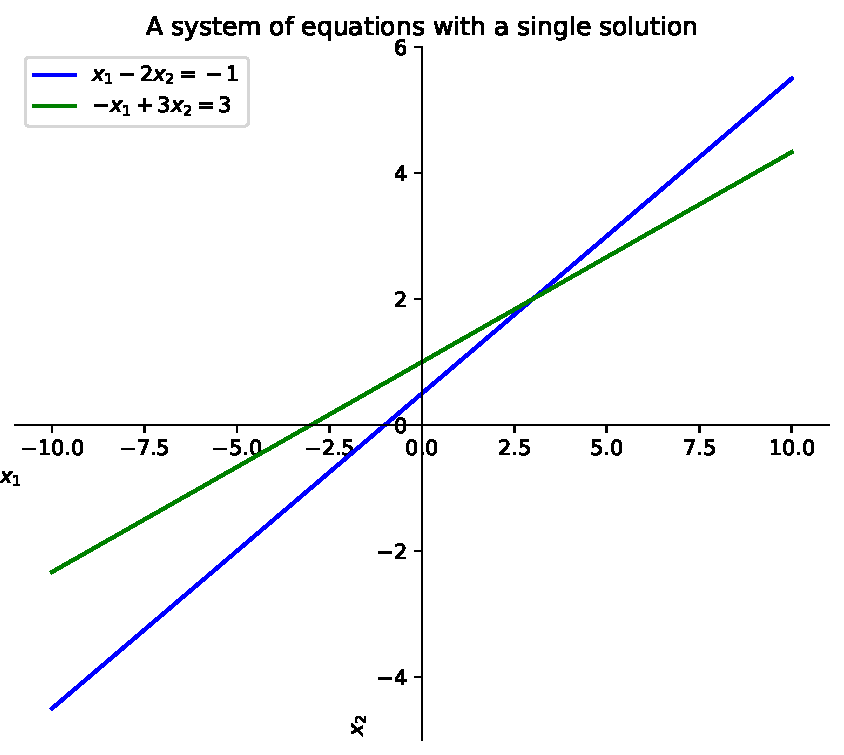
\includegraphics{p1_files/figure-pdf/cell-3-output-1.pdf}

}

\end{figure}

\begin{tcolorbox}[enhanced jigsaw, colbacktitle=quarto-callout-note-color!10!white, toprule=.15mm, colback=white, breakable, titlerule=0mm, leftrule=.75mm, bottomtitle=1mm, opacitybacktitle=0.6, bottomrule=.15mm, title=\textcolor{quarto-callout-note-color}{\faInfo}\hspace{0.5em}{Definition of a system of linear equations}, left=2mm, colframe=quarto-callout-note-color-frame, rightrule=.15mm, toptitle=1mm, opacityback=0, arc=.35mm, coltitle=black]

A system of linear equations (or a linear system) is a collection of one
or more linear equations involving the same variables- say
\(x_1, x_2, \ldots, x_n\). An example is

\[
\begin{cases}
&x_1 &- 2x_2 &= -1\\
-&x_1 &+ 3x_2 &= 3
\end{cases}
\]

The above system has two equations and two variables where \(x_1, x_2\)
are the variables.

\end{tcolorbox}

The equations above have only one solution since they intersect at a
single point.

\begin{Shaded}
\begin{Highlighting}[]
\ImportTok{from}\NormalTok{ IPython.display }\ImportTok{import}\NormalTok{ Markdown}

\NormalTok{solution }\OperatorTok{=}\NormalTok{ sp.solve((equation\_1, equation\_2), (x1, x2))}
\NormalTok{Markdown(}\SpecialStringTok{f\textquotesingle{}$$}\CharTok{\textbackslash{}n}\SpecialCharTok{\{}\NormalTok{sp}\SpecialCharTok{.}\NormalTok{latex(solution)}\SpecialCharTok{\}}\CharTok{\textbackslash{}n}\SpecialStringTok{$$\textquotesingle{}}\NormalTok{)}
\end{Highlighting}
\end{Shaded}

\[
\left\{ x_{1} : 3, \  x_{2} : 2\right\}
\]

\begin{Shaded}
\begin{Highlighting}[]
\ImportTok{import}\NormalTok{ sympy }\ImportTok{as}\NormalTok{ sp}
\ImportTok{import}\NormalTok{ matplotlib.pyplot }\ImportTok{as}\NormalTok{ plt}
\ImportTok{import}\NormalTok{ numpy }\ImportTok{as}\NormalTok{ np}

\NormalTok{x1, x2 }\OperatorTok{=}\NormalTok{ sp.symbols(}\StringTok{\textquotesingle{}x\_1 x\_2\textquotesingle{}}\NormalTok{)}

\NormalTok{equation\_1 }\OperatorTok{=}\NormalTok{ sp.Eq(x1 }\OperatorTok{{-}} \DecValTok{2}\OperatorTok{*}\NormalTok{x2, }\OperatorTok{{-}}\DecValTok{1}\NormalTok{)}
\NormalTok{graph\_eq1 }\OperatorTok{=}\NormalTok{ sp.solve(equation\_1, x2)[}\DecValTok{0}\NormalTok{]}

\NormalTok{equation\_2 }\OperatorTok{=}\NormalTok{ sp.Eq(}\OperatorTok{{-}}\NormalTok{x1 }\OperatorTok{+} \DecValTok{3}\OperatorTok{*}\NormalTok{x2, }\DecValTok{3}\NormalTok{)}
\NormalTok{graph\_eq2 }\OperatorTok{=}\NormalTok{ sp.solve(equation\_2, x2)[}\DecValTok{0}\NormalTok{]}

\CommentTok{\# Generate data for plotting}
\NormalTok{x1\_vals }\OperatorTok{=}\NormalTok{ np.linspace(}\OperatorTok{{-}}\DecValTok{10}\NormalTok{, }\DecValTok{10}\NormalTok{, }\DecValTok{400}\NormalTok{)}
\NormalTok{graph\_eq1\_lambdified }\OperatorTok{=}\NormalTok{ sp.lambdify(x1, graph\_eq1)}
\NormalTok{graph\_eq2\_lambdified }\OperatorTok{=}\NormalTok{ sp.lambdify(x1, graph\_eq2)}
\NormalTok{y1\_vals }\OperatorTok{=}\NormalTok{ graph\_eq1\_lambdified(x1\_vals)}
\NormalTok{y2\_vals }\OperatorTok{=}\NormalTok{ graph\_eq2\_lambdified(x1\_vals)}

\CommentTok{\# Plotting}
\NormalTok{fig, ax }\OperatorTok{=}\NormalTok{ plt.subplots(figsize}\OperatorTok{=}\NormalTok{(}\DecValTok{7}\NormalTok{, }\DecValTok{6}\NormalTok{))}

\NormalTok{ax.set\_title(}\StringTok{\textquotesingle{}A system of equations with a single solution\textquotesingle{}}\NormalTok{)}
\NormalTok{ax.set\_xlabel(}\StringTok{\textquotesingle{}$x\_1$                                                                                                                            \textquotesingle{}}\NormalTok{)}
\NormalTok{ax.set\_ylabel(}\StringTok{\textquotesingle{}$x\_2$                                                                                                    \textquotesingle{}}\NormalTok{)}

\CommentTok{\# Plot the equations}
\NormalTok{ax.plot(x1\_vals, y1\_vals, label}\OperatorTok{=}\StringTok{\textquotesingle{}$x\_1 {-} 2x\_2 = {-}1$\textquotesingle{}}\NormalTok{, color}\OperatorTok{=}\StringTok{\textquotesingle{}blue\textquotesingle{}}\NormalTok{)}
\NormalTok{ax.plot(x1\_vals, y2\_vals, label}\OperatorTok{=}\StringTok{\textquotesingle{}${-}x\_1 + 3x\_2 = 3$\textquotesingle{}}\NormalTok{, color}\OperatorTok{=}\StringTok{\textquotesingle{}green\textquotesingle{}}\NormalTok{)}

\CommentTok{\# Move the left and bottom spines to x = 0 and y = 0, respectively}
\NormalTok{ax.spines[}\StringTok{\textquotesingle{}left\textquotesingle{}}\NormalTok{].set\_position(}\StringTok{\textquotesingle{}zero\textquotesingle{}}\NormalTok{)}
\NormalTok{ax.spines[}\StringTok{\textquotesingle{}bottom\textquotesingle{}}\NormalTok{].set\_position(}\StringTok{\textquotesingle{}zero\textquotesingle{}}\NormalTok{)}
\NormalTok{ax.spines[}\StringTok{\textquotesingle{}right\textquotesingle{}}\NormalTok{].set\_color(}\StringTok{\textquotesingle{}none\textquotesingle{}}\NormalTok{)}
\NormalTok{ax.spines[}\StringTok{\textquotesingle{}top\textquotesingle{}}\NormalTok{].set\_color(}\StringTok{\textquotesingle{}none\textquotesingle{}}\NormalTok{)}

\CommentTok{\# Plot the solution}
\NormalTok{solution }\OperatorTok{=}\NormalTok{ sp.solve((equation\_1, equation\_2), (x1, x2))}
\NormalTok{solution\_x1 }\OperatorTok{=}\NormalTok{ solution[x1]}
\NormalTok{solution\_x2 }\OperatorTok{=}\NormalTok{ solution[x2]}

\NormalTok{ax.scatter([solution\_x1], [solution\_x2], color}\OperatorTok{=}\StringTok{\textquotesingle{}red\textquotesingle{}}\NormalTok{, zorder}\OperatorTok{=}\DecValTok{3}\NormalTok{)  }
\NormalTok{ax.text(solution\_x1}\OperatorTok{+}\FloatTok{.5}\NormalTok{, solution\_x2}\OperatorTok{{-}}\FloatTok{.5}\NormalTok{, }\StringTok{\textquotesingle{}  Solution\textquotesingle{}}\NormalTok{, fontsize}\OperatorTok{=}\DecValTok{12}\NormalTok{)}

\CommentTok{\# Add legend and grid}
\NormalTok{ax.legend()}
\NormalTok{plt.show()}
\end{Highlighting}
\end{Shaded}

\begin{figure}[H]

{\centering 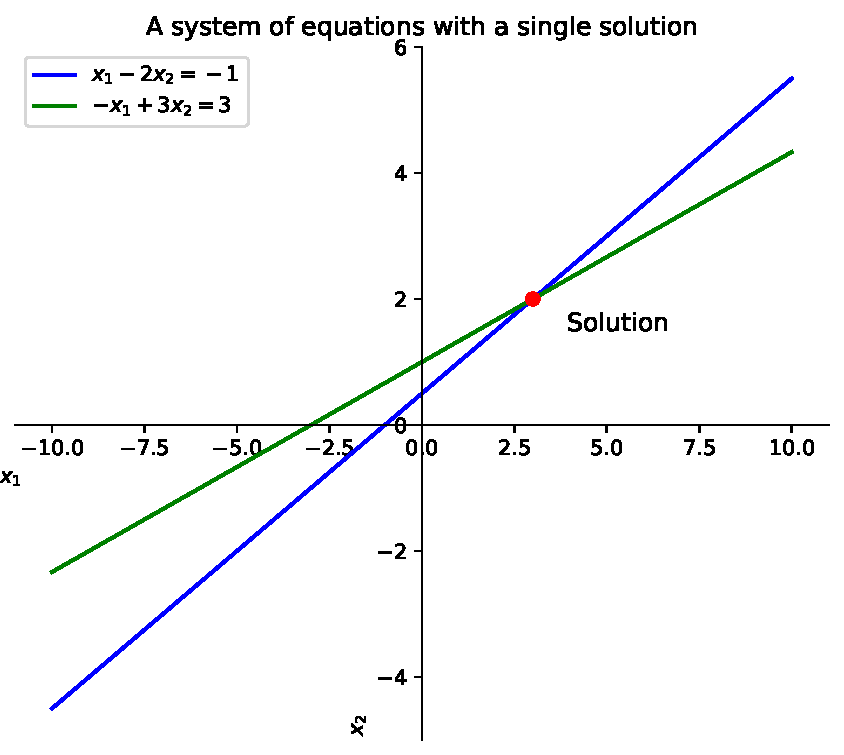
\includegraphics{p1_files/figure-pdf/cell-5-output-1.pdf}

}

\end{figure}

\begin{tcolorbox}[enhanced jigsaw, colbacktitle=quarto-callout-note-color!10!white, toprule=.15mm, colback=white, breakable, titlerule=0mm, leftrule=.75mm, bottomtitle=1mm, opacitybacktitle=0.6, bottomrule=.15mm, title=\textcolor{quarto-callout-note-color}{\faInfo}\hspace{0.5em}{Definition of a solution}, left=2mm, colframe=quarto-callout-note-color-frame, rightrule=.15mm, toptitle=1mm, opacityback=0, arc=.35mm, coltitle=black]

A solution of a linear system is a list of numbers
(\(s_1, s_2, \ldots, s_n\)) that makes each equation a true statement
when the values \(s_1, s_2, \ldots, s_n\) are substituted for
\(x_1, x_2, \ldots, x_n\), respectively.

For example, the list of numbers, \((3,2)\), is a solution of the system
above because, when the values \(3,2\) are substituted for \(x_1, x_2\),
respectively, both equations are a true statement.

\end{tcolorbox}

The above list, \((3,2)\), is the solution to the system of equations
because it is the only list of numbers that makes both equations true.
When we substitute \(3\) and \(2\) for \(x_1\) and \(x_2\) in the first
equation, both equations turn out to be true!

\[
\begin{cases}
&x_1 &- 2x_2 &= -1\\
-&x_1 &+ 3x_2 &= 3
\end{cases}
\]

turns into

\[
\begin{cases}
&(3) &- 2(2) &= -1 \;\; &\text{True!}\\
-&(3) &+ 3(2) &= 3 \;\; &\text{True!}
\end{cases}
\]

\hypertarget{systems-without-a-single-solution}{%
\subsection*{Systems without a Single
Solution}\label{systems-without-a-single-solution}}
\addcontentsline{toc}{subsection}{Systems without a Single Solution}

\hypertarget{no-solution}{%
\paragraph*{\texorpdfstring{\textbf{No
Solution}}{No Solution}}\label{no-solution}}
\addcontentsline{toc}{paragraph}{\textbf{No Solution}}

Take the following system of linear equations:

\[
\begin{cases}
&x_1 &- 2x_2 &= -1\\
-&x_1 &+ 2x_2 &= 3
\end{cases}
\]

If we plot these equations on a graph, we can see that they are parallel
and never intersect. This means that there is no solution to this system
of equations.

\begin{Shaded}
\begin{Highlighting}[]
\ImportTok{import}\NormalTok{ sympy }\ImportTok{as}\NormalTok{ sp}
\ImportTok{import}\NormalTok{ matplotlib.pyplot }\ImportTok{as}\NormalTok{ plt}
\ImportTok{import}\NormalTok{ numpy }\ImportTok{as}\NormalTok{ np}

\NormalTok{x1, x2 }\OperatorTok{=}\NormalTok{ sp.symbols(}\StringTok{\textquotesingle{}x\_1 x\_2\textquotesingle{}}\NormalTok{)}

\CommentTok{\# Define the equations}
\NormalTok{equation\_1 }\OperatorTok{=}\NormalTok{ sp.Eq(x1 }\OperatorTok{{-}} \DecValTok{2}\OperatorTok{*}\NormalTok{x2, }\OperatorTok{{-}}\DecValTok{1}\NormalTok{)}
\NormalTok{graph\_eq1 }\OperatorTok{=}\NormalTok{ sp.solve(equation\_1, x2)[}\DecValTok{0}\NormalTok{]}

\NormalTok{equation\_2 }\OperatorTok{=}\NormalTok{ sp.Eq(}\OperatorTok{{-}}\NormalTok{x1 }\OperatorTok{+} \DecValTok{2}\OperatorTok{*}\NormalTok{x2, }\DecValTok{3}\NormalTok{)}
\NormalTok{graph\_eq2 }\OperatorTok{=}\NormalTok{ sp.solve(equation\_2, x2)[}\DecValTok{0}\NormalTok{]}

\CommentTok{\# Generate data for plotting}
\NormalTok{x1\_vals }\OperatorTok{=}\NormalTok{ np.linspace(}\OperatorTok{{-}}\DecValTok{10}\NormalTok{, }\DecValTok{10}\NormalTok{, }\DecValTok{400}\NormalTok{)}
\NormalTok{graph\_eq1\_lambdified }\OperatorTok{=}\NormalTok{ sp.lambdify(x1, graph\_eq1)}
\NormalTok{graph\_eq2\_lambdified }\OperatorTok{=}\NormalTok{ sp.lambdify(x1, graph\_eq2)}
\NormalTok{y1\_vals }\OperatorTok{=}\NormalTok{ graph\_eq1\_lambdified(x1\_vals)}
\NormalTok{y2\_vals }\OperatorTok{=}\NormalTok{ graph\_eq2\_lambdified(x1\_vals)}

\CommentTok{\# Plotting}
\NormalTok{fig, ax }\OperatorTok{=}\NormalTok{ plt.subplots(figsize}\OperatorTok{=}\NormalTok{(}\DecValTok{7}\NormalTok{, }\DecValTok{6}\NormalTok{))}

\NormalTok{ax.set\_title(}\StringTok{\textquotesingle{}A system of equations with no solution\textquotesingle{}}\NormalTok{)}
\NormalTok{ax.set\_xlabel(}\StringTok{\textquotesingle{}$x\_1$                                                                                                                            \textquotesingle{}}\NormalTok{)}
\NormalTok{ax.set\_ylabel(}\StringTok{\textquotesingle{}$x\_2$                                                                                                    \textquotesingle{}}\NormalTok{)}

\CommentTok{\# Plot the equations}
\NormalTok{ax.plot(x1\_vals, y1\_vals, label}\OperatorTok{=}\StringTok{\textquotesingle{}$x\_1 {-} 2x\_2 = {-}1$\textquotesingle{}}\NormalTok{, color}\OperatorTok{=}\StringTok{\textquotesingle{}blue\textquotesingle{}}\NormalTok{)}
\NormalTok{ax.plot(x1\_vals, y2\_vals, label}\OperatorTok{=}\StringTok{\textquotesingle{}${-}x\_1 + 2x\_2 = 3$\textquotesingle{}}\NormalTok{, color}\OperatorTok{=}\StringTok{\textquotesingle{}green\textquotesingle{}}\NormalTok{)}

\CommentTok{\# Move the left and bottom spines to x = 0 and y = 0, respectively}
\NormalTok{ax.spines[}\StringTok{\textquotesingle{}left\textquotesingle{}}\NormalTok{].set\_position(}\StringTok{\textquotesingle{}zero\textquotesingle{}}\NormalTok{)}
\NormalTok{ax.spines[}\StringTok{\textquotesingle{}bottom\textquotesingle{}}\NormalTok{].set\_position(}\StringTok{\textquotesingle{}zero\textquotesingle{}}\NormalTok{)}
\NormalTok{ax.spines[}\StringTok{\textquotesingle{}right\textquotesingle{}}\NormalTok{].set\_color(}\StringTok{\textquotesingle{}none\textquotesingle{}}\NormalTok{)}
\NormalTok{ax.spines[}\StringTok{\textquotesingle{}top\textquotesingle{}}\NormalTok{].set\_color(}\StringTok{\textquotesingle{}none\textquotesingle{}}\NormalTok{)}

\CommentTok{\# Add legend and grid}
\NormalTok{ax.legend()}
\NormalTok{plt.show()}
\end{Highlighting}
\end{Shaded}

\begin{figure}[H]

{\centering 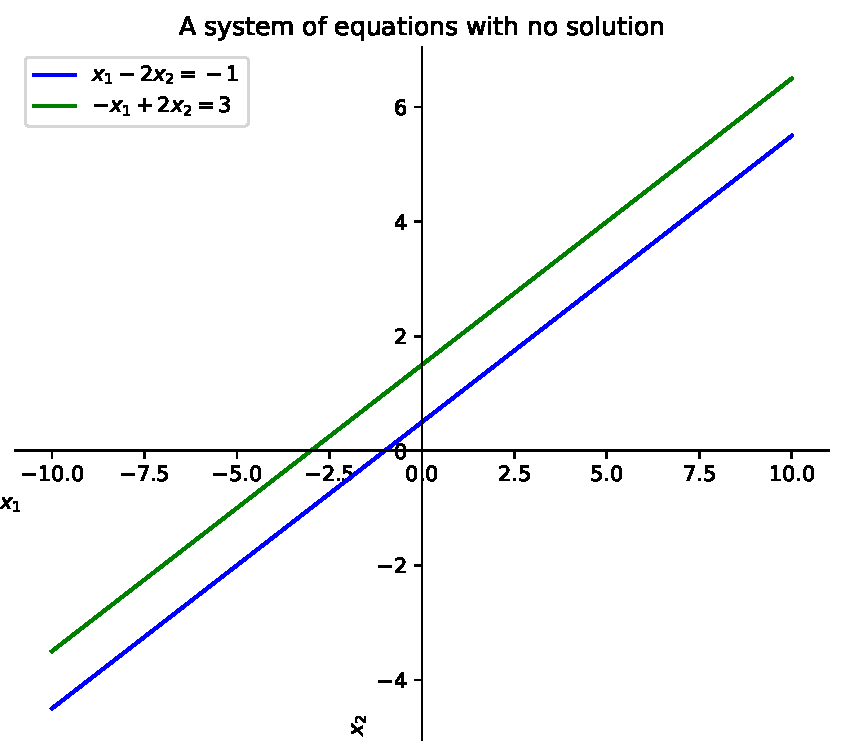
\includegraphics{p1_files/figure-pdf/cell-6-output-1.pdf}

}

\end{figure}

\hypertarget{infinite-solutions}{%
\paragraph*{\texorpdfstring{\textbf{Infinite
Solutions}}{Infinite Solutions}}\label{infinite-solutions}}
\addcontentsline{toc}{paragraph}{\textbf{Infinite Solutions}}

Take the following system of linear equations:

\[
\begin{cases}
&x_1 &- 2x_2 &= -1\\
-&x_1 &+ 2x_2 &= 1
\end{cases}
\]

If we plot these equations on a graph, we can see that they are the same
line. This means that there are an infinite number of solutions to this
system of equations.

\begin{Shaded}
\begin{Highlighting}[]
\ImportTok{import}\NormalTok{ sympy }\ImportTok{as}\NormalTok{ sp}
\ImportTok{import}\NormalTok{ matplotlib.pyplot }\ImportTok{as}\NormalTok{ plt}
\ImportTok{import}\NormalTok{ numpy }\ImportTok{as}\NormalTok{ np}

\NormalTok{x1, x2 }\OperatorTok{=}\NormalTok{ sp.symbols(}\StringTok{\textquotesingle{}x\_1 x\_2\textquotesingle{}}\NormalTok{)}

\CommentTok{\# Define the equations}
\NormalTok{equation\_1 }\OperatorTok{=}\NormalTok{ sp.Eq(x1 }\OperatorTok{{-}} \DecValTok{2}\OperatorTok{*}\NormalTok{x2, }\OperatorTok{{-}}\DecValTok{1}\NormalTok{)}
\NormalTok{graph\_eq1 }\OperatorTok{=}\NormalTok{ sp.solve(equation\_1, x2)[}\DecValTok{0}\NormalTok{]}

\NormalTok{equation\_2 }\OperatorTok{=}\NormalTok{ sp.Eq(}\OperatorTok{{-}}\NormalTok{x1 }\OperatorTok{+} \DecValTok{2}\OperatorTok{*}\NormalTok{x2, }\DecValTok{1}\NormalTok{)}
\NormalTok{graph\_eq2 }\OperatorTok{=}\NormalTok{ sp.solve(equation\_2, x2)[}\DecValTok{0}\NormalTok{]}

\CommentTok{\# Generate data for plotting}
\NormalTok{x1\_vals }\OperatorTok{=}\NormalTok{ np.linspace(}\OperatorTok{{-}}\DecValTok{10}\NormalTok{, }\DecValTok{10}\NormalTok{, }\DecValTok{400}\NormalTok{)}
\NormalTok{graph\_eq1\_lambdified }\OperatorTok{=}\NormalTok{ sp.lambdify(x1, graph\_eq1)}
\NormalTok{graph\_eq2\_lambdified }\OperatorTok{=}\NormalTok{ sp.lambdify(x1, graph\_eq2)}
\NormalTok{y1\_vals }\OperatorTok{=}\NormalTok{ graph\_eq1\_lambdified(x1\_vals)}
\NormalTok{y2\_vals }\OperatorTok{=}\NormalTok{ graph\_eq2\_lambdified(x1\_vals)}

\CommentTok{\# Plotting}
\NormalTok{fig, ax }\OperatorTok{=}\NormalTok{ plt.subplots(figsize}\OperatorTok{=}\NormalTok{(}\DecValTok{7}\NormalTok{, }\DecValTok{6}\NormalTok{))}

\NormalTok{ax.set\_title(}\StringTok{\textquotesingle{}A system of equations with infinite solutions\textquotesingle{}}\NormalTok{)}
\NormalTok{ax.set\_xlabel(}\StringTok{\textquotesingle{}$x\_1$                                                                                                                            \textquotesingle{}}\NormalTok{)}
\NormalTok{ax.set\_ylabel(}\StringTok{\textquotesingle{}$x\_2$                                                                                                    \textquotesingle{}}\NormalTok{)}

\CommentTok{\# Plot the equations}
\NormalTok{ax.plot(x1\_vals, y1\_vals, label}\OperatorTok{=}\StringTok{\textquotesingle{}$x\_1 {-} 2x\_2 = {-}1$\textquotesingle{}}\NormalTok{, color}\OperatorTok{=}\StringTok{\textquotesingle{}blue\textquotesingle{}}\NormalTok{)}
\NormalTok{ax.plot(x1\_vals, y2\_vals, label}\OperatorTok{=}\StringTok{\textquotesingle{}${-}x\_1 + 2x\_2 = 1$\textquotesingle{}}\NormalTok{, color}\OperatorTok{=}\StringTok{\textquotesingle{}green\textquotesingle{}}\NormalTok{, linestyle}\OperatorTok{=}\StringTok{\textquotesingle{}dashed\textquotesingle{}}\NormalTok{)}

\CommentTok{\# Move the left and bottom spines to x = 0 and y = 0, respectively}
\NormalTok{ax.spines[}\StringTok{\textquotesingle{}left\textquotesingle{}}\NormalTok{].set\_position(}\StringTok{\textquotesingle{}zero\textquotesingle{}}\NormalTok{)}
\NormalTok{ax.spines[}\StringTok{\textquotesingle{}bottom\textquotesingle{}}\NormalTok{].set\_position(}\StringTok{\textquotesingle{}zero\textquotesingle{}}\NormalTok{)}
\NormalTok{ax.spines[}\StringTok{\textquotesingle{}right\textquotesingle{}}\NormalTok{].set\_color(}\StringTok{\textquotesingle{}none\textquotesingle{}}\NormalTok{)}
\NormalTok{ax.spines[}\StringTok{\textquotesingle{}top\textquotesingle{}}\NormalTok{].set\_color(}\StringTok{\textquotesingle{}none\textquotesingle{}}\NormalTok{)}

\CommentTok{\# Add legend and grid}
\NormalTok{ax.legend()}
\NormalTok{plt.show()}
\end{Highlighting}
\end{Shaded}

\begin{figure}[H]

{\centering 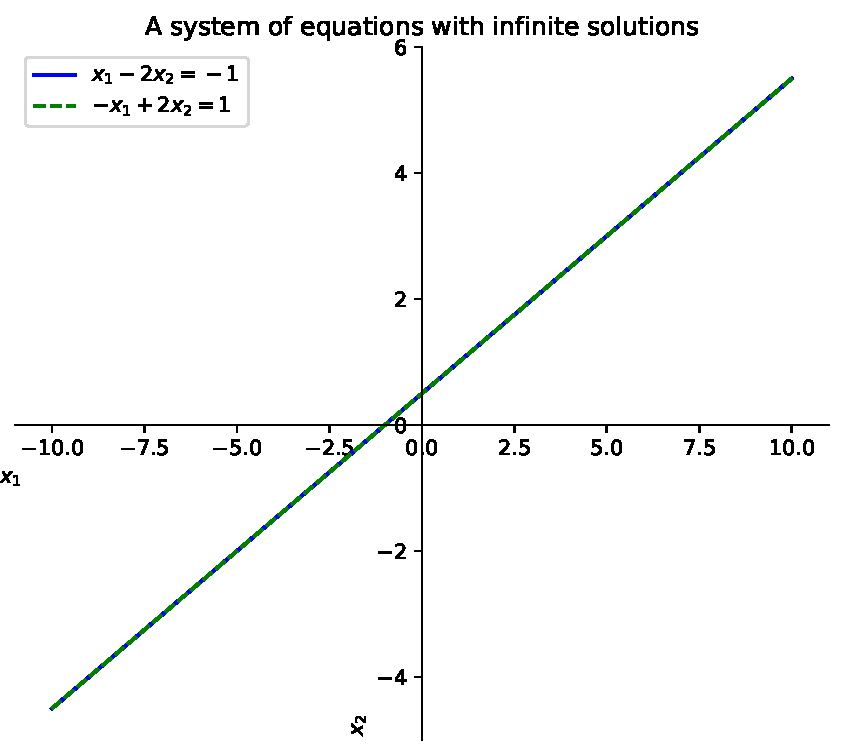
\includegraphics{p1_files/figure-pdf/cell-7-output-1.pdf}

}

\end{figure}

\begin{tcolorbox}[enhanced jigsaw, colbacktitle=quarto-callout-tip-color!10!white, toprule=.15mm, colback=white, breakable, titlerule=0mm, leftrule=.75mm, bottomtitle=1mm, opacitybacktitle=0.6, bottomrule=.15mm, title=\textcolor{quarto-callout-tip-color}{\faLightbulb}\hspace{0.5em}{Tip}, left=2mm, colframe=quarto-callout-tip-color-frame, rightrule=.15mm, toptitle=1mm, opacityback=0, arc=.35mm, coltitle=black]

A system of linear equations has

\begin{enumerate}
\def\labelenumi{\arabic{enumi}.}
\tightlist
\item
  no solution, or
\item
  exactly one solution, or
\item
  infinitely many solutions.
\end{enumerate}

\end{tcolorbox}

\bookmarksetup{startatroot}

\hypertarget{matrix-notation}{%
\chapter*{Matrix Notation}\label{matrix-notation}}
\addcontentsline{toc}{chapter}{Matrix Notation}

\markboth{Matrix Notation}{Matrix Notation}

\hypertarget{converting-a-system-of-linear-equations-to-matrix-form}{%
\section*{Converting a system of linear equations to matrix
form}\label{converting-a-system-of-linear-equations-to-matrix-form}}
\addcontentsline{toc}{section}{Converting a system of linear equations
to matrix form}

\markright{Converting a system of linear equations to matrix form}

The essential information of a linear system can be recorded compactly
in a rectangular array called a matrix.

The following system of linear equations:

\[
\begin{cases}
&x_1 &- 2x_2 &= -1\\
-&x_1 &+ 3x_2 &= 3
\end{cases}
\]

The following matrix is called the \textbf{coefficient matrix} of the
system, it contains the coefficients of the variables left of the equals
sign:

\[
\begin{bmatrix}
1 & -2\\
-1 & 3
\end{bmatrix}
\]

The following matrix is called the \textbf{augmented matrix} of the
system, it contains the coefficients of the variables left of the equals
sign and the constants right of the equals sign (separated by a vertical
line):

\[
\begin{bmatrix}
1 & -2 &|& -1\\
-1 & 3 &|& 3
\end{bmatrix}
\]

\hypertarget{dimensions-of-a-matrix}{%
\section*{Dimensions of a matrix:}\label{dimensions-of-a-matrix}}
\addcontentsline{toc}{section}{Dimensions of a matrix:}

\markright{Dimensions of a matrix:}

The size of a matrix tells how many rows and columns it has. The
augmented matrix above has 3 rows and 4 columns and is called a
\(3 \times 4\) (read ``3 by 4'') matrix.

If m and n are positive integers, an m n matrix is a rectangular array
of numbers with m rows and n columns. (The number of rows always comes
first.) Matrix notation will simplify the calculations in the examples
that follow

\begin{tcolorbox}[enhanced jigsaw, colbacktitle=quarto-callout-tip-color!10!white, toprule=.15mm, colback=white, breakable, titlerule=0mm, leftrule=.75mm, bottomtitle=1mm, opacitybacktitle=0.6, bottomrule=.15mm, title=\textcolor{quarto-callout-tip-color}{\faLightbulb}\hspace{0.5em}{Tip}, left=2mm, colframe=quarto-callout-tip-color-frame, rightrule=.15mm, toptitle=1mm, opacityback=0, arc=.35mm, coltitle=black]

In matrix notation:

\begin{itemize}
\tightlist
\item
  \(m\) is the number of rows
\item
  \(n\) is the number of columns
\end{itemize}

\end{tcolorbox}

\bookmarksetup{startatroot}

\hypertarget{row-reduction-and-echelon-forms}{%
\chapter{Row Reduction and Echelon
Forms}\label{row-reduction-and-echelon-forms}}

A matrix has a few different ``special'' forms. Two specific forms are
the \textbf{row echelon form} and the \textbf{reduced row echelon form}.
These forms are useful because they make it easy to solve systems of
linear equations. Below we will build up to these forms by discussing
the elements of a matrix, types of forms, and the elementary row
operations that are used to reduce a matrix to these forms.

\hypertarget{elements-of-a-matrix}{%
\section*{Elements of a matrix}\label{elements-of-a-matrix}}
\addcontentsline{toc}{section}{Elements of a matrix}

\markright{Elements of a matrix}

Check out the following matrix:

\[
\left[\begin{array}{ccc}
    1 & 2 & 3 & 4 \\
    0 & 5 & 6 & 7 \\
    0 & 0 & 0 & 8 \\
    0 & 0 & 0 & 0
\end{array}\right]
\begin{array}{c}
    \leftarrow R_1 \\
    \leftarrow R_2 \\
    \leftarrow R_3 \\
    \leftarrow R_4
\end{array}
\]

\hypertarget{leading-entries}{%
\subsection*{Leading Entries}\label{leading-entries}}
\addcontentsline{toc}{subsection}{Leading Entries}

The \textbf{leading entry} of a row is the first nonzero entry in that
row. For example,

\begin{itemize}
\tightlist
\item
  the leading entry of \(R_1\) is 1,
\item
  the leading entry of \(R_2\) is 5,\\
\item
  the leading entry of \(R_3\) is 8, and
\item
  \(R_4\) has no leading entry.
\end{itemize}

\hypertarget{pivot-positions}{%
\subsection*{Pivot Positions}\label{pivot-positions}}
\addcontentsline{toc}{subsection}{Pivot Positions}

The \textbf{pivot positions} of a matrix are the positions of the
leading entries in the matrix.

\begin{itemize}
\tightlist
\item
  for \(R_1\), the leading entry is in the first column,
\item
  for \(R_2\) the leading entry is in the second column,\\
\item
  for \(R_3\), the leading entry is in the fourth column, and
\item
  \(R_4\) has no leading entry- thus no pivot position.
\end{itemize}

\hypertarget{zero-rows}{%
\subsection*{Zero Rows}\label{zero-rows}}
\addcontentsline{toc}{subsection}{Zero Rows}

A \textbf{zero row} is a row that contains only zeros. In the example
above, \(R_4\) is a zero row.

\hypertarget{row-echelon-form}{%
\section*{Row Echelon Form}\label{row-echelon-form}}
\addcontentsline{toc}{section}{Row Echelon Form}

\markright{Row Echelon Form}

A matrix is in \textbf{row echelon form} if it meets the following
criteria:

\begin{enumerate}
\def\labelenumi{\arabic{enumi}.}
\tightlist
\item
  Zero rows are at the bottom of the matrix.
\item
  Each leading entry of a row is in a column to the right of the leading
  entry of the row above it.
\item
  All entries in a column below a leading entry are zeros.
\end{enumerate}

Here are some examples of matrices in row echelon form:

\chapter{Square}

\[
\begin{bmatrix}
    1 & 2 & 3 \\
    0 & 4 & 5 \\
    0 & 0 & 6 
\end{bmatrix}
\]

\chapter{Tall (m \textgreater{} n)}

\[
\begin{bmatrix}
    2 & 3 & 4 \\
    0 & 1 & 5 \\
    0 & 0 & 3 \\
    0 & 0 & 0
\end{bmatrix}
\]

\chapter{Wide (m \textless{} n)}

\[
\begin{bmatrix}
  1 & 2 & 3 & 4 \\
  0 & 0 & 0 & 0 \\
  0 & 0 & 0 & 0
\end{bmatrix}
\]

\chapter{General Form (sorta)}

\[
\begin{bmatrix}
    \square & * & * & \dots & * \\
    0 & \square & * & \dots & * \\
    0 & 0 & \square & \dots & * \\
    \vdots & \vdots & \vdots & \ddots & \vdots \\
    0 & 0 & 0 & \dots & \square \\
    0 & 0 & 0 & \dots & 0
\end{bmatrix}
\]

where \(\square\) represents a nonzero entry, and \(*\) represents any
entry (possibly zero).

\hypertarget{reduced-row-echelon-form}{%
\section*{Reduced Row Echelon Form}\label{reduced-row-echelon-form}}
\addcontentsline{toc}{section}{Reduced Row Echelon Form}

\markright{Reduced Row Echelon Form}

A matrix is in \textbf{reduced row echelon form} if it meets the
following criteria:

\begin{enumerate}
\def\labelenumi{\arabic{enumi}.}
\tightlist
\item
  It is in row echelon form.
\item
  The leading entry in each nonzero row is 1.
\item
  Each leading 1 is the only nonzero entry in its column.
\end{enumerate}

Here are some examples of matrices in reduced row echelon form:

\chapter{Square}

\[
\begin{bmatrix}
    1 & 0 & 0 \\
    0 & 1 & 0 \\
    0 & 0 & 1 
\end{bmatrix}
\]

\chapter{Tall (m \textgreater{} n)}

\[
\begin{bmatrix}
    1 & 0 & 0 \\
    0 & 1 & 0 \\
    0 & 0 & 1 \\
    0 & 0 & 0
\end{bmatrix}
\]

\chapter{Wide (m \textless{} n)}

\[
\begin{bmatrix}
  1 & 0 & 0 & 1 \\
  0 & 1 & 0 & 2 \\
  0 & 0 & 1 & 3
\end{bmatrix}
\]

\chapter{General Form (sorta)}

\[
\begin{bmatrix}
    1 & 0 & \dots & 0 & * \\
    0 & 1 & \dots & 0 & * \\
    \vdots & \vdots & \ddots & \vdots & \vdots \\
    0 & 0 & \dots & 1 & * \\
    0 & 0 & \dots & 0 & 0
\end{bmatrix}
\]

\hypertarget{elementary-row-operations}{%
\section*{Elementary Row Operations}\label{elementary-row-operations}}
\addcontentsline{toc}{section}{Elementary Row Operations}

\markright{Elementary Row Operations}

There are three types of elementary row operations:

\begin{enumerate}
\def\labelenumi{\arabic{enumi}.}
\tightlist
\item
  \textbf{Swap the positions of two rows.}
\end{enumerate}

\[
R_i \leftrightarrow R_j
\]

\begin{enumerate}
\def\labelenumi{\arabic{enumi}.}
\setcounter{enumi}{1}
\tightlist
\item
  \textbf{Multiply a row by a non-zero scalar.}
\end{enumerate}

\[
kR_i \rightarrow R_i
\]

\begin{enumerate}
\def\labelenumi{\arabic{enumi}.}
\setcounter{enumi}{2}
\tightlist
\item
  \textbf{Add or subtract the multiple of one row to another row.}
\end{enumerate}

\[
kR_i + R_j \rightarrow R_j
\]

\hypertarget{the-row-reduction-algorithm}{%
\section*{The Row Reduction
Algorithm}\label{the-row-reduction-algorithm}}
\addcontentsline{toc}{section}{The Row Reduction Algorithm}

\markright{The Row Reduction Algorithm}

The \textbf{row reduction algorithm} is a method for solving systems of
linear equations. It is based on the idea that if two systems of
equations have the same solution, then the augmented matrices of those
systems are row equivalent. This means that the two matrices can be
transformed into each other by a sequence of elementary row operations.
The row reduction algorithm is used to transform a matrix into row
echelon form or reduced row echelon form.

\hypertarget{the-forward-phase}{%
\subsection*{The Forward Phase}\label{the-forward-phase}}
\addcontentsline{toc}{subsection}{The Forward Phase}

The forward phase of the row reduction algorithm is used to reduce a
matrix to row echelon form. The steps are as follows:

\begin{enumerate}
\def\labelenumi{\arabic{enumi}.}
\tightlist
\item
  Write the augmented matrix of the system of equations.
\item
  Begin with the leftmost nonzero column. This is a pivot column. The
  pivot position is at the top. Select a nonzero entry in the pivot
  column as a pivot. If necessary, interchange rows to move this entry
  into the pivot position
\item
  Use row replacement operations to create zeros in all positions below
  the pivot
\item
  Assuming all the entries under the last pivot is zero, we can now
  ignore the row containing the pivot position and cover all rows, if
  any, above it. Apply steps 1-3 to the remaining submatrix. Repeat the
  process until there are no more nonzero rows to modify.
\end{enumerate}

\chapter{Step 1}

Below is the augmented matrix of a system of equations.

\[
\begin{bmatrix}
    0 & 3 & -6 & 6 \\
    3 & -7 & 8 & -5 \\
    3 & -9 & 12 & -9
\end{bmatrix}
\]

\chapter{Step 2}

Step 2 states: \emph{Begin with the leftmost nonzero column. This is a
pivot column. The pivot position is at the top. Select a nonzero entry
in the pivot column as a pivot. If necessary, interchange rows to move
this entry into the pivot position.}

\[
\begin{bmatrix}
    \mathbf{0} & 3 & -6 & 6 \\
    \mathbf{3} & -7 & 8 & -5 \\
    \mathbf{3} & -9 & 12 & -9
\end{bmatrix}
\]

Since the first entry in \(R_1\) is a zero, we need to swap it with a
row where the first entry is not a zero. We can swap \(R_1\) with
\(R_2\) or \(R_3\).

\[
\begin{array}{c}
     R_1 \rightarrow \\
     R_2 \rightarrow \\
     R_3 \rightarrow \\
\end{array}
\left[\begin{array}{ccc}
    \mathbf{0} & 3 & -6 & 6 \\
    \mathbf{3} & -7 & 8 & -5 \\
    \mathbf{3} & -9 & 12 & -9
\end{array}\right]
\]

We can do the following:

\(R_1 \leftrightarrow R_2 \;\;\;\) or \(\;\;\;R_1 \leftrightarrow R_3\)

I guess, let's do \(R_1 \leftrightarrow R_2\)\ldots{}

Since we did an elementary row operation, we need to update our matrix
into a new matrix:

\[
\begin{bmatrix}
    \mathbf{0} & 3 & -6 & 6 \\
    \mathbf{3} & -7 & 8 & -5 \\
    \mathbf{3} & -9 & 12 & -9
\end{bmatrix}
\]

\[
\downarrow
\]

\[
\begin{bmatrix}
    \mathbf{3} & -7 & 8 & -5  \\
    \mathbf{0} & 3 & -6 & 6   \\
    \mathbf{3} & -9 & 12 & -9
\end{bmatrix}
\]

\chapter{Step 3}

Step 3 states: \emph{Use row replacement operations to create zeros in
all positions below the pivot.}

\[
\begin{array}{c}
    R_1\rightarrow\\
    R_2\rightarrow\\
    R_3\rightarrow\\
\end{array}
\left[\begin{array}{ccc}
    \mathbf{3} & -7 & 8 & -5  \\
    \mathbf{0} & 3 & -6 & 6   \\
    \mathbf{3} & -9 & 12 & -9
\end{array}\right]
\]

The bottom left number \(3\) in \(R_3\) needs fixing since it is a
non-zero entry below the pivot that we're working with. We can do the
elementary row operation: \emph{Add or subtract the multiple of one row
to another row} to fix this. \[
kR_i + R_j \rightarrow R_j
\]

\[
\text{where } k = -1, i = 1, \text{ and } j = 3
\]

\[
-R_1 + R_3 \rightarrow R_2
\]

The operation is performed as follows:

\[
-R_1
\]

\[
\begin{align*}
    &(-1)\left[ -3,  \;-7, \;\; 8, \;\;\; -5 \right] \\
\end{align*}
\]

\[
\downarrow
\]

\[
\begin{align*}
    &\left[ (-1)3,  \;(-1)-7, \;\; (-1)8, \;\;\; (-1)-5 \right] \\
\end{align*}
\]

\[
\downarrow
\]

\[
\begin{bmatrix}
    -3, \;\;7, -8, \;\;5
\end{bmatrix}
\]

\[
R_3
\]

\[
\begin{bmatrix}
    3 & -9 & 12 & -9 \\
\end{bmatrix}
\]

Below is what happens when we add the two rows together:

\[
-R_1 + R_2
\]

\[
\downarrow
\]

\[
\begin{array}{cc}
    &\left[\;-3,  \;\;\;\;7, \;\; -8, \;\;\;\; 5 \right] \\
    +\; &\left[ \;\;\;3, \;\; -9, \;\;\;12, \; -9 \right]
\end{array}
\]

\[
\rule{6cm}{0.4pt}
\]

\[
=\;\;\;\;\;\begin{bmatrix}
    \;\;0 & -2 & \;\;4 & -4 \\
\end{bmatrix}
\]

Now, \(\left[0 \; -2 \;\; 4 -4 \right]\) is the new \(R_2\).

New matrix:

\[
\begin{bmatrix}
    3 & -9 & 12 & -9 \\
    0 & 3 & -6 & 6 \\
    0 & -2 & 4 & -4
\end{bmatrix}
\]

\chapter{Step 4}

Step 4 states: \emph{Assuming all the entries under the last pivot is
zero, we can now ignore the row containing the pivot position and cover
all rows, if any, above it. Apply steps 1-3 to the remaining submatrix.
Repeat the process until there are no more nonzero rows to modify.}

Below, we can see that all the entries under the last pivot are zero, so
we can ignore the row containing the pivot position and cover all rows,
if any, above it.

\[
\begin{bmatrix}
    \bf{3} & -9 & 12 & -9 \\
    \bf{0} & 3 & -6 & 6 \\
    \bf{0} & 2 & 4 & 4
\end{bmatrix}
\]

\[
\text{Since everything below the 3 is a zero,}
\]

\[
\begin{array}{c}
    \text{we can ignore the first row now} \rightarrow \\
                                \\
                                \\
\end{array}
\begin{bmatrix}
    \times & \times & \times & \times \\
    0 & \bf{3} & -6 & 6 \\
    0 & \bf{-2} & 4 & -4
\end{bmatrix}
\]

We can now apply steps 1-3 to the remaining submatrix. Repeat the
process until finished.

\[
\begin{array}{c}
    R_1 \rightarrow \\
    R_2 \rightarrow \\
    R_3 \rightarrow \\
\end{array}
\begin{bmatrix}
    3 & -9 & 12 & -9 \\
    0 & 3 & -6 & 6 \\
    0 & -2 & 4 & -4
\end{bmatrix}
\]

\[
\downarrow
\]

\[
\frac{2}{3}R_2 + R_3 \rightarrow R_3
\]

\[
\downarrow
\]

\[
\begin{bmatrix}
    3 & -9 & 12 & -9 \\
    0 & 3 & -6 & 6 \\
    0 & 0 & 0 & 0
\end{bmatrix}
\]

\chapter{Finish}

We can now see that the matrix is in row echelon form.

\[
\begin{bmatrix}
    3 & -9 & 12 & -9 \\
    0 & 3 & -6 & 6 \\
    0 & 0 & 0 & 0
\end{bmatrix}
\]

If we were to solve this with python, we would do the following:

\begin{Shaded}
\begin{Highlighting}[]
\ImportTok{import}\NormalTok{ sympy }\ImportTok{as}\NormalTok{ sp  }
\ImportTok{from}\NormalTok{ sympy }\ImportTok{import}\NormalTok{ init\_printing}
\NormalTok{init\_printing()}

\NormalTok{A }\OperatorTok{=}\NormalTok{ sp.Matrix([}
\NormalTok{    [}\DecValTok{0}\NormalTok{,  }\DecValTok{3}\NormalTok{,  }\OperatorTok{{-}}\DecValTok{6}\NormalTok{,   }\DecValTok{6}\NormalTok{], }
\NormalTok{    [}\DecValTok{3}\NormalTok{, }\OperatorTok{{-}}\DecValTok{7}\NormalTok{,   }\DecValTok{8}\NormalTok{,  }\OperatorTok{{-}}\DecValTok{5}\NormalTok{], }
\NormalTok{    [}\DecValTok{3}\NormalTok{, }\OperatorTok{{-}}\DecValTok{9}\NormalTok{,  }\DecValTok{12}\NormalTok{,  }\OperatorTok{{-}}\DecValTok{9}\NormalTok{]])}

\NormalTok{A.echelon\_form()}
\end{Highlighting}
\end{Shaded}

\begin{figure}[H]

{\centering 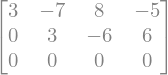
\includegraphics{p2_files/figure-pdf/cell-2-output-1.png}

}

\end{figure}

\emph{Note that depending on step 2, we could have swapped \(R_1\) with
\(R_3\) instead of \(R_1\) with \(R_2\). This would have resulted in a
different matrix}

\hypertarget{the-backwards-phase}{%
\subsection*{The Backwards Phase}\label{the-backwards-phase}}
\addcontentsline{toc}{subsection}{The Backwards Phase}

The backwards phase of the row reduction algorithm is used to reduce a
matrix in row echelon form to reduced row echelon form. The
\textbf{reduced row echelon form} of a matrix is unique. This means that
there is only one reduced row echelon form for a given matrix. This is
not true for row echelon form. A matrix can have many different row
echelon forms. The steps are as follows:

\begin{enumerate}
\def\labelenumi{\arabic{enumi}.}
\setcounter{enumi}{4}
\tightlist
\item
  Beginning with the rightmost pivot and working upward and to the left,
  create zeros above each pivot. If a pivot is not 1, make it 1 by a
  scaling operation.
\end{enumerate}

\chapter{Step 5a}

Step five says: \emph{Beginning with the rightmost pivot and working
upward and to the left, create zeros above each pivot. If a pivot is not
1, make it 1 by a scaling operation.}

Below is the matrix from the previous example in row echelon form.
Currently the only pivots are 3 and 3. We can make the rightmost pivot 1
by dividing the row by 3.

\[
\begin{bmatrix}
    \bf{3} & -9 & 12 & -9 \\
    0 & \bf{3} & -6 & 6 \\
    0 & 0 & 0 & 0
\end{bmatrix}
\]

\[
\downarrow
\]

\[
\frac{1}{3}R_2 \rightarrow R_2
\]

\[
\downarrow
\]

\[
\begin{bmatrix}
    \bf{3} & -9 & 12 & -9 \\
    0 & \bf{1} & -2 & 2 \\
    0 & 0 & 0 & 0
\end{bmatrix}
\]

\chapter{Step 5b}

For the right most pivot, we can make the entries above it zero with
elementary row operations.

\[
\begin{bmatrix}
    3 & -9 & 12 & -9 \\
    0 & \bf{1} & -2 & 2 \\
    0 & 0 & 0 & 0
\end{bmatrix}
\]

\[
\downarrow
\]

\[
9R_2 + R_1 \rightarrow R_1
\]

\[
\downarrow
\]

\[
\begin{bmatrix}
    3 & 0 & -6 & 9 \\
    0 & \bf{1} & -2 & 2 \\
    0 & 0 & 0 & 0
\end{bmatrix}
\]

\chapter{Step 5c}

Now we can make the leftmost pivot 1 by dividing the row by 3.

\[
\begin{bmatrix}
    3 & 0 & -6 & 9 \\
    0 & \bf{1} & -2 & 2 \\
    0 & 0 & 0 & 0
\end{bmatrix}
\]

\[
\downarrow
\]

\[
\frac{1}{3}R_1 \rightarrow R_1
\]

\[
\downarrow
\]

\[
\begin{bmatrix}
    1 & 0 & -2 & 3 \\
    0 & 1 & -2 & 2 \\
    0 & 0 & 0 & 0
\end{bmatrix}
\]

\chapter{Finish}

We can now see that the matrix is in reduced row echelon form.

\[
\begin{bmatrix}
    1 & 0 & -2 & 3 \\
    0 & 1 & -2 & 2 \\
    0 & 0 & 0 & 0
\end{bmatrix}
\]

Alternatively, we can solve this with python:

\begin{Shaded}
\begin{Highlighting}[]
\ImportTok{import}\NormalTok{ sympy }\ImportTok{as}\NormalTok{ sp  }
\ImportTok{from}\NormalTok{ sympy }\ImportTok{import}\NormalTok{ init\_printing}
\NormalTok{init\_printing()}

\NormalTok{A }\OperatorTok{=}\NormalTok{ sp.Matrix([}
\NormalTok{    [}\DecValTok{0}\NormalTok{,  }\DecValTok{3}\NormalTok{,  }\OperatorTok{{-}}\DecValTok{6}\NormalTok{,   }\DecValTok{6}\NormalTok{], }
\NormalTok{    [}\DecValTok{3}\NormalTok{, }\OperatorTok{{-}}\DecValTok{7}\NormalTok{,   }\DecValTok{8}\NormalTok{,  }\OperatorTok{{-}}\DecValTok{5}\NormalTok{], }
\NormalTok{    [}\DecValTok{3}\NormalTok{, }\OperatorTok{{-}}\DecValTok{9}\NormalTok{,  }\DecValTok{12}\NormalTok{,  }\OperatorTok{{-}}\DecValTok{9}\NormalTok{]])}

\NormalTok{A.rref()[}\DecValTok{0}\NormalTok{]}
\end{Highlighting}
\end{Shaded}

\begin{figure}[H]

{\centering 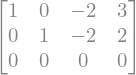
\includegraphics{p2_files/figure-pdf/cell-3-output-1.png}

}

\end{figure}

\begin{Shaded}
\begin{Highlighting}[]
\ImportTok{import}\NormalTok{ sympy }\ImportTok{as}\NormalTok{ sp  }
\ImportTok{from}\NormalTok{ sympy }\ImportTok{import}\NormalTok{ init\_printing}
\NormalTok{init\_printing()}

\NormalTok{A }\OperatorTok{=}\NormalTok{ sp.Matrix([}
\NormalTok{    [}\DecValTok{3}\NormalTok{, }\OperatorTok{{-}}\DecValTok{9}\NormalTok{,  }\DecValTok{12}\NormalTok{,  }\OperatorTok{{-}}\DecValTok{9}\NormalTok{], }
\NormalTok{    [}\DecValTok{0}\NormalTok{,  }\DecValTok{3}\NormalTok{,  }\OperatorTok{{-}}\DecValTok{6}\NormalTok{,   }\DecValTok{6}\NormalTok{],}
\NormalTok{    [}\DecValTok{0}\NormalTok{,  }\DecValTok{0}\NormalTok{,   }\DecValTok{0}\NormalTok{,   }\DecValTok{0}\NormalTok{]])}

\NormalTok{A.rref()[}\DecValTok{0}\NormalTok{]}
\end{Highlighting}
\end{Shaded}

\begin{figure}[H]

{\centering 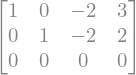
\includegraphics{p2_files/figure-pdf/cell-4-output-1.png}

}

\end{figure}

\bookmarksetup{startatroot}

\hypertarget{solving-linear-systems}{%
\chapter{Solving Linear Systems}\label{solving-linear-systems}}

\begin{tcolorbox}[enhanced jigsaw, colbacktitle=quarto-callout-note-color!10!white, toprule=.15mm, colback=white, breakable, titlerule=0mm, leftrule=.75mm, bottomtitle=1mm, opacitybacktitle=0.6, bottomrule=.15mm, title=\textcolor{quarto-callout-note-color}{\faInfo}\hspace{0.5em}{Existence and Uniqueness Question}, left=2mm, colframe=quarto-callout-note-color-frame, rightrule=.15mm, toptitle=1mm, opacityback=0, arc=.35mm, coltitle=black]

The two fundamental questions about a linear system are:

\begin{enumerate}
\def\labelenumi{\arabic{enumi}.}
\tightlist
\item
  Is the system consistent; that is, does at least one solution exist?
\item
  If a solution exists, is it the only one; that is, is the solution
  unique
\end{enumerate}

\textbf{Examples from \href{./p1.html}{Linear Systems (page 1)}}

A consistent system that has a unique solution

\[
\left[\begin{array}{cc|c}
1 & -2 & -1 \\
-1 & 3 & 3
\end{array}\right]
\]

A consistent system that has infinitely many solutions

\[
\left[\begin{array}{cc|c}
1 & -2 & -1 \\
-1 & 2 & 1
\end{array}\right]  
\]

An inconsistent system (A system that has no solution)

\[
\left[\begin{array}{cc|c}
1 & -2 & -1 \\
-1 & 2 & 3
\end{array}\right]
\]

\end{tcolorbox}

\hypertarget{the-workflow-for-solving-a-linear-system}{%
\section*{The workflow for solving a linear
system}\label{the-workflow-for-solving-a-linear-system}}
\addcontentsline{toc}{section}{The workflow for solving a linear system}

\markright{The workflow for solving a linear system}

\begin{enumerate}
\def\labelenumi{\arabic{enumi}.}
\tightlist
\item
  The linear system is written out in a system of equations.
\item
  Convert the system of equations to an augmented matrix.
\item
  Use elementary row operations to reduce the matrix to row echelon
  form.
\item
  Convert the reduced row echelon form back to a system of equations.
\end{enumerate}

\hypertarget{infinitely-many-solutions-example}{%
\subsection*{Infinitely Many Solutions
Example}\label{infinitely-many-solutions-example}}
\addcontentsline{toc}{subsection}{Infinitely Many Solutions Example}

\chapter{Step 1}

\begin{enumerate}
\def\labelenumi{\arabic{enumi}.}
\tightlist
\item
  The linear system is written out in a system of equations.
\end{enumerate}

Here is a linear system written as a system of equations.

\[
\begin{cases}
&\;\;x_1 &- &3x_2 &+ &4x_3 &= -4 \\
&3x_1 &- &7x_2 &+ &7x_3 &= -8 \\
&2x_1 &- &6x_2 &- &8x_3 &= -8
\end{cases}
\]

\chapter{Step 2}

\begin{enumerate}
\def\labelenumi{\arabic{enumi}.}
\setcounter{enumi}{1}
\tightlist
\item
  Convert the system of equations to an augmented matrix.
\end{enumerate}

The system of equations is converted to an augmented matrix.

\[
\begin{cases}
&\;\;x_1 &- &3x_2 &+ &4x_3 &= -4 \\
&3x_1 &- &7x_2 &+ &7x_3 &= -8 \\
&2x_1 &- &6x_2 &- &8x_3 &= -8
\end{cases}
\]

\[
\downarrow
\]

\[
\left[\begin{array}{ccc|c}
1 & -3 & 4 & -4 \\
3 & -7 & 7 & -8 \\
2 & -6 & -8 & -8
\end{array}\right]
\]

\chapter{Step 3}

\begin{enumerate}
\def\labelenumi{\arabic{enumi}.}
\setcounter{enumi}{2}
\tightlist
\item
  Use elementary row operations to reduce the matrix to row echelon
  form.
\end{enumerate}

\[
\left[\begin{array}{ccc|c}
1 & -3 & 4 & -4 \\
3 & -7 & 7 & -8 \\
2 & -6 & -8 & -8
\end{array}\right]
\]

\[
\downarrow
\]

\begin{Shaded}
\begin{Highlighting}[]
\ImportTok{import}\NormalTok{ sympy }\ImportTok{as}\NormalTok{ sp}
\ImportTok{from}\NormalTok{ sympy }\ImportTok{import}\NormalTok{ init\_printing}
\NormalTok{init\_printing()}

\NormalTok{A }\OperatorTok{=}\NormalTok{ sp.Matrix([}
\NormalTok{    [}\DecValTok{1}\NormalTok{, }\OperatorTok{{-}}\DecValTok{3}\NormalTok{, }\DecValTok{4}\NormalTok{, }\OperatorTok{{-}}\DecValTok{4}\NormalTok{],}
\NormalTok{    [}\DecValTok{3}\NormalTok{, }\OperatorTok{{-}}\DecValTok{7}\NormalTok{, }\DecValTok{7}\NormalTok{, }\OperatorTok{{-}}\DecValTok{8}\NormalTok{],}
\NormalTok{    [}\DecValTok{2}\NormalTok{, }\OperatorTok{{-}}\DecValTok{6}\NormalTok{, }\DecValTok{8}\NormalTok{, }\OperatorTok{{-}}\DecValTok{8}\NormalTok{]}
\NormalTok{])}

\NormalTok{A.echelon\_form()}
\end{Highlighting}
\end{Shaded}

\begin{figure}[H]

{\centering 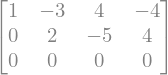
\includegraphics{p3_files/figure-pdf/cell-2-output-1.png}

}

\end{figure}

\chapter{Step 4}

\begin{enumerate}
\def\labelenumi{\arabic{enumi}.}
\setcounter{enumi}{3}
\tightlist
\item
  Convert the reduced row echelon form back to a system of equations.
\end{enumerate}

\[
\displaystyle \left[\begin{matrix}1 & -3 & 4 & -4\\0 & 2 & -5 & 4\\0 & 0 & 0 & 0\end{matrix}\right]
\]

\[
\downarrow
\]

\[
\begin{cases}
x_1 &- &3x_2 &+ &4x_3 &= -4 \\
& &\;\;2x_2 &- &5x_3 &= \;\;\;4 \\
& & & &0x_3 &= \;\;\;0
\end{cases}
\]

\chapter{Finish}

The system of equations is written out as so:

\[
\begin{cases}
x_1 &- &3x_2 &+ &4x_3 &= -4 \\
& &2x_2 &- &5x_3 &= \;\;\;4 \\
& & & &0x_3 &= \;\;\;0
\end{cases}
\]

We can see that the system is consistent because the last equation is
\(0x_3 = 0\) which is always true. Therefore, the system has infinitely
many solutions.

\hypertarget{no-solution-example}{%
\subsection*{No Solution Example}\label{no-solution-example}}
\addcontentsline{toc}{subsection}{No Solution Example}

\chapter{Step 1}

\begin{enumerate}
\def\labelenumi{\arabic{enumi}.}
\tightlist
\item
  The linear system is written out in a system of equations.
\end{enumerate}

Here is a linear system written as a system of equations.

\[
\begin{cases}
& & &\;\;x_2 &+ &4x_3 &= -5 \\
&\;\;x_1 &- &3x_2 &+ &5x_3 &= -2 \\
&3x_1 &+ &7x_2 &+ &7x_3 &= \;\;\;6
\end{cases}
\]

\chapter{Step 2}

\begin{enumerate}
\def\labelenumi{\arabic{enumi}.}
\setcounter{enumi}{1}
\tightlist
\item
  Convert the system of equations to an augmented matrix.
\end{enumerate}

The system of equations is converted to an augmented matrix.

\[
\begin{cases}
& & &\;\;x_2 &+ &4x_3 &= -5 \\
&\;\;x_1 &- &3x_2 &+ &5x_3 &= -2 \\
&3x_1 &+ &7x_2 &+ &7x_3 &= \;\;\;6
\end{cases}
\]

\[
\downarrow
\]

\[
\left[\begin{array}{ccc|c}
0 & 1 & 4 & -5 \\
1 & 3 & 5 & -2 \\
3 & 7 & 7 & 6
\end{array}\right]
\]

\chapter{Step 3}

\begin{enumerate}
\def\labelenumi{\arabic{enumi}.}
\setcounter{enumi}{2}
\tightlist
\item
  Use elementary row operations to reduce the matrix to row echelon
  form.
\end{enumerate}

\[
\left[\begin{array}{ccc|c}
0 & 1 & 4 & -5 \\
1 & 3 & 5 & -2 \\
3 & 7 & 7 & 6
\end{array}\right]
\]

\[
\downarrow
\]

\begin{Shaded}
\begin{Highlighting}[]
\ImportTok{import}\NormalTok{ sympy }\ImportTok{as}\NormalTok{ sp  }
\ImportTok{from}\NormalTok{ sympy }\ImportTok{import}\NormalTok{ init\_printing}
\NormalTok{init\_printing()}

\NormalTok{A }\OperatorTok{=}\NormalTok{ sp.Matrix([}
\NormalTok{    [}\DecValTok{0}\NormalTok{, }\DecValTok{1}\NormalTok{, }\DecValTok{4}\NormalTok{, }\OperatorTok{{-}}\DecValTok{5}\NormalTok{],}
\NormalTok{    [}\DecValTok{1}\NormalTok{, }\DecValTok{3}\NormalTok{, }\DecValTok{5}\NormalTok{, }\OperatorTok{{-}}\DecValTok{2}\NormalTok{],}
\NormalTok{    [}\DecValTok{3}\NormalTok{, }\DecValTok{7}\NormalTok{, }\DecValTok{7}\NormalTok{, }\DecValTok{6}\NormalTok{]}
\NormalTok{])}

\NormalTok{A.echelon\_form()}
\end{Highlighting}
\end{Shaded}

\begin{figure}[H]

{\centering 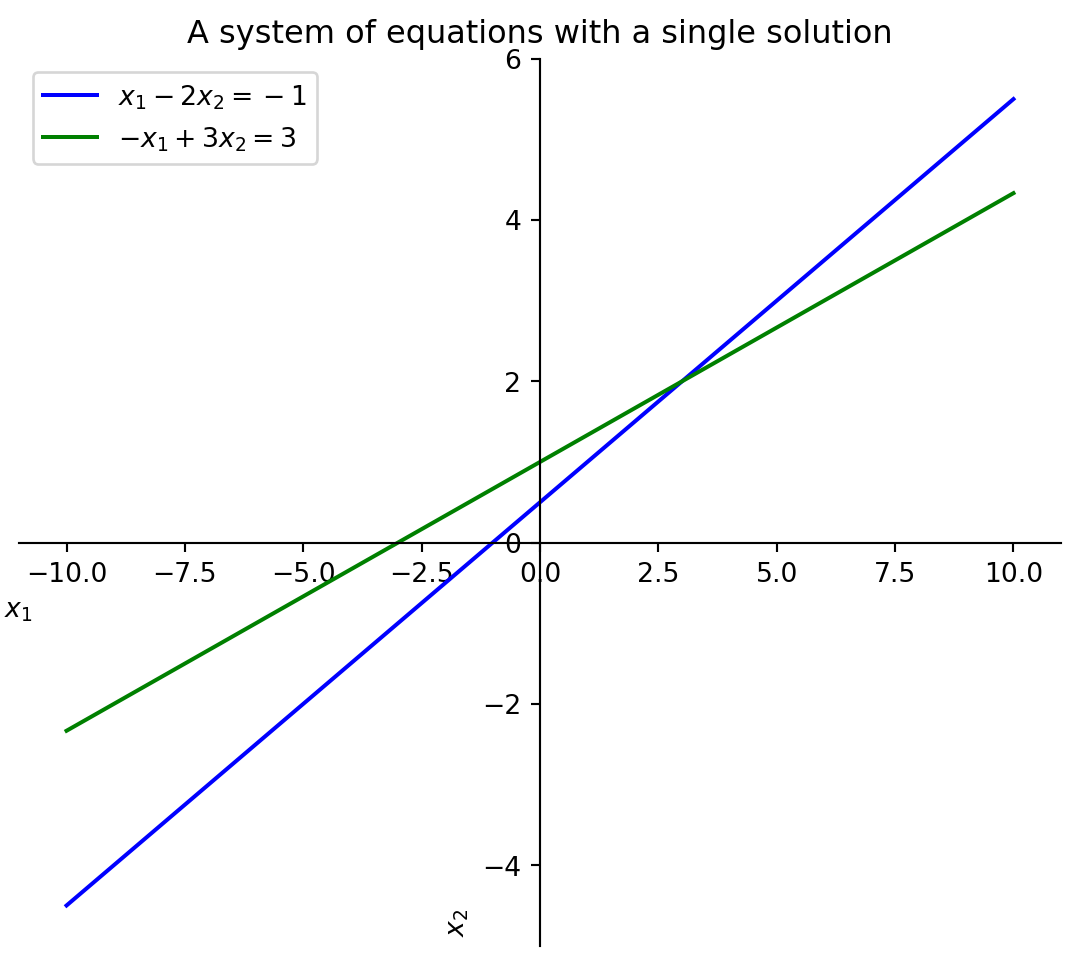
\includegraphics{p3_files/figure-pdf/cell-3-output-1.png}

}

\end{figure}

\chapter{Step 4}

\begin{enumerate}
\def\labelenumi{\arabic{enumi}.}
\setcounter{enumi}{3}
\tightlist
\item
  Convert the reduced row echelon form back to a system of equations.
\end{enumerate}

\[
\displaystyle \left[\begin{matrix}1 & 3 & 5 & -2\\0 & 1 & 4 & -5\\0 & 0 & 0 & 2\end{matrix}\right]
\]

\[  
\downarrow
\]

\[
\begin{cases}
x_1 &+ &3x_2 &+ &5x_3 &= -2 \\
& &\;\;x_2 &+ &4x_3 &= -5 \\
& & & &0x_3 &= \;\;\;2
\end{cases}
\]

\chapter{Finish}

The system of equations is written out as so:

\[
\begin{cases}
x_1 &+ &3x_2 &+ &5x_3 &= -2 \\
& &\;\;x_2 &+ &4x_3 &= -5 \\
& & & &0x_3 &= \;\;\;2
\end{cases}
\]

We can see that the system is inconsistent because the last equation is
\(0x_3 = 2\) which is impossible. No value of \(x_3\) will make this
equation true. Therefore, the system has no solution.

\bookmarksetup{startatroot}

\hypertarget{vectors}{%
\chapter{Vectors}\label{vectors}}

\bookmarksetup{startatroot}

\hypertarget{references}{%
\chapter*{References}\label{references}}
\addcontentsline{toc}{chapter}{References}

\markboth{References}{References}

\hypertarget{refs}{}
\begin{CSLReferences}{0}{0}
\end{CSLReferences}



\end{document}
